% Plantilla IETAGRO Puerto Giraldo — 1° PARTE (1S) PERSONALIZADA
% =================================================================
% Mantiene EXACTAMENTE la misma geometría del archivo original:
%   - Posición de los 4 marcadores fiduciales (8mm desde cada esquina)
%   - Posición de los timing marks por fila
%   - Posición de las burbujas (4 columnas en el mismo Y)
%   - Caja del título de 2.4 cm de alto (de y=-2.1 a y=-4.5)
%   - Espaciado vertical entre header y columnas
%
% Modificaciones únicamente VISUALES en el header (sin cambiar tamaños):
%   - Pre-impresión del nombre y documento (sin escritura manual)
%   - Línea de documento acortada (de 6cm a 3cm)
%   - Etiqueta "DOC. IDENT." abreviada (en lugar de "DOCUMENTO IDENTIDAD")
%   - QR de 22mm × 22mm en el espacio liberado a la derecha
%   - Línea adicional con CURSO y SESIÓN debajo del logo
%
% Placeholders (rellenados por Python antes de compilar):
%   <<NOMBRE>>   Nombres y apellidos del estudiante (mayúsculas)
%   <<ID>>       Documento de identidad
%   <<CURSO>>    Curso (ej. 11A)
%   <<QR_PATH>>  Ruta absoluta del PNG del QR

\documentclass[letterpaper]{article}
\usepackage[top=1.1cm, bottom=0.9cm, left=1.2cm, right=1.1cm]{geometry}
\usepackage{tikz}
\usepackage{graphicx}
\usetikzlibrary{calc, shapes.geometric, positioning}
\usepackage[T1]{fontenc}
\usepackage[utf8]{inputenc}
\usepackage{helvet}
\renewcommand{\familydefault}{\sfdefault}
\setlength{\parindent}{0pt}
\setlength{\parskip}{0pt}
\pagestyle{empty}

%================= AJUSTE FINO OMR (idéntico al original) =================
\newlength{\TMw}    \setlength{\TMw}{6pt}
\newlength{\Nw}     \setlength{\Nw}{14pt}
\newlength{\Bdia}   \setlength{\Bdia}{12pt}
\newlength{\Bsep}   \setlength{\Bsep}{1.5pt}
\newlength{\Brad}   \setlength{\Brad}{6pt}
\newlength{\Rowsep} \setlength{\Rowsep}{2pt}

\tikzset{cuadrocolumna/.style={
    draw, draw=black!70, line width=1.2pt,
    rounded corners=10pt, inner sep=8pt, outer sep=0pt,
    fill=white, align=left, anchor=north,
    text width=\linewidth-16pt
}}

\newcommand{\B}{%
  \makebox[\Bdia][c]{%
    \tikz[baseline=-2.8pt]{%
      \filldraw[fill=white, draw=black!70, line width=0.7pt, rounded corners=0pt, solid]
        (0,0) circle (\Brad);}%
  }%
}

\newcommand{\TM}{%
  \makebox[\TMw][c]{%
    \tikz[baseline=-4pt]{\fill[black, rounded corners=0pt, solid](0,-5pt) rectangle (\TMw,5pt);}%
  }%
}

\newcommand{\Q}[1]{%
  \noindent
  \TM\hspace{1pt}%
  \makebox[\Nw][r]{\scriptsize\textbf{#1.}}%
  \hspace{2pt}%
  \B\hspace{\Bsep}\B\hspace{\Bsep}\B\hspace{\Bsep}\B%
  \par\vspace{\Rowsep}%
}

\newcommand{\QH}[1]{%
  \noindent
  \TM\hspace{1pt}%
  \makebox[\Nw][r]{\scriptsize\textbf{#1.}}%
  \hspace{2pt}%
  \B\hspace{\Bsep}\B\hspace{\Bsep}\B\hspace{\Bsep}\B\hspace{\Bsep}%
  \B\hspace{\Bsep}\B\hspace{\Bsep}\B\hspace{\Bsep}\B%
  \par\vspace{\Rowsep}%
}

\newcommand{\HDR}{%
  \noindent
  \hspace{\TMw}\hspace{1pt}\hspace{\Nw}\hspace{2pt}%
  \foreach \L in {A,B,C,D}{%
    \makebox[\Bdia][c]{\footnotesize\textbf{\L}}\hspace{\Bsep}%
  }%
  \par\vspace{2pt}%
}

\newcommand{\HDRH}{%
  \noindent
  \hspace{\TMw}\hspace{1pt}\hspace{\Nw}\hspace{2pt}%
  \foreach \L in {A,B,C,D,E,F,G,H}{%
    \makebox[\Bdia][c]{\footnotesize\textbf{\L}}\hspace{\Bsep}%
  }%
  \par\vspace{2pt}%
}

\begin{document}

%================= MARCADORES DE PÁGINA (IDÉNTICOS al original) =================
\begin{tikzpicture}[remember picture, overlay]
  \fill[black] ($(current page.north west)+(8mm,-8mm)$)  rectangle ++(8mm,-8mm);
  \fill[black] ($(current page.north east)+(-8mm,-8mm)$) rectangle ++(-8mm,-8mm);
  \fill[black] ($(current page.south west)+(8mm,16mm)$)  rectangle ++(8mm,8mm);
  \fill[black] ($(current page.south east)+(-8mm,16mm)$) rectangle ++(-8mm,8mm);
\end{tikzpicture}

\vspace*{2mm}

% ================== ENCABEZADO PRINCIPAL ==================
% Misma caja (2.4cm de alto), mismo posicionamiento que el original.
\noindent\makebox[\textwidth][c]{
\begin{tikzpicture}[x=1cm, y=1cm]

% --- Caja principal (IDÉNTICA al original: -2.1 a -4.5) ---
\draw[line width=2pt, rounded corners=10pt] (-9, -2.1) rectangle (9, -4.5);

% --- Título (font \large en lugar de \Large para dejar espacio al QR) ---
\node[font=\large\bfseries, align=center] at (-1.0, -2.45)
  {SIMULACRO SABER 11° - 1° PARTE};

% --- IZQUIERDA: Nombre del estudiante PRE-IMPRESO + línea original ---
\node[font=\normalsize, anchor=south] at (-4.75, -3.36) {<<NOMBRE>>};
\draw[line width=1.5pt] (-8, -3.4) -- (-1.5, -3.4);
\node[font=\normalsize\bfseries] at (-4.55, -3.9) {NOMBRES Y APELLIDOS};

% --- CENTRO: Logo "Pruebas Saber 11°" (IDÉNTICO al original) ---
\begin{scope}[shift={(0, -3.4)}]
    \fill[black] (-1.3, 0.7) -- (-0.9, 0.3) -- (-0.5, 0.7) -- (-0.5, 0.45) -- (-0.9, 0.05) -- (-1.3, 0.45) -- cycle;
    \fill[black] (-1.3, 0.3) -- (-0.9, -0.1) -- (-0.5, 0.3) -- (-0.5, 0.05) -- (-0.9, -0.35) -- (-1.3, 0.05) -- cycle;
    \node[anchor=west, align=left, inner sep=0] at (-0.3, 0.2) {\fontsize{6}{7}\selectfont Pruebas\\[-0.5ex]\large\bfseries Saber};
    \fill[black!90] (1.6, 0.2) circle (0.45);
    \node[text=white, font=\bfseries\normalsize] at (1.6, 0.2) {11$^\circ$};
\end{scope}

% --- DOCUMENTO: ID PRE-IMPRESO + línea acortada (3cm en lugar de 6cm) ---
\node[font=\normalsize, anchor=south] at (4.0, -3.36) {<<ID>>};
\draw[line width=1.5pt] (2.5, -3.4) -- (5.5, -3.4);
\node[font=\normalsize\bfseries] at (4.0, -3.9) {DOC. IDENT.};

% --- DERECHA: QR de 22mm × 22mm en el espacio liberado ---
% Centro vertical de la caja (entre y=-2.1 y y=-4.5 → y=-3.3)
% El QR (22mm) ocupa de y=-2.2 a y=-4.4 → CABE dentro de la caja (1mm margen arriba/abajo)
\node[anchor=center, inner sep=0] at (7.5, -3.3) {%
  \includegraphics[width=22mm]{<<QR_PATH>>}};

% --- CURSO + SESIÓN: dentro de la caja, debajo del logo y el doc ---
\node[font=\scriptsize\bfseries, anchor=west] at (-0.5, -4.25) {CURSO:};
\node[font=\normalsize\bfseries, anchor=west] at (0.9, -4.25) {<<CURSO>>};
\node[font=\scriptsize\bfseries, anchor=west] at (2.3, -4.25) {SES.:};
\node[font=\normalsize\bfseries, anchor=west] at (3.3, -4.25) {1S};

\end{tikzpicture}
}

\vspace{6mm}

%================= RESPUESTAS (POSICIONES IDÉNTICAS al original) =================
\noindent
% Columna 1
\begin{minipage}[t]{0.20\textwidth}
  \vspace{0pt}
  \noindent
  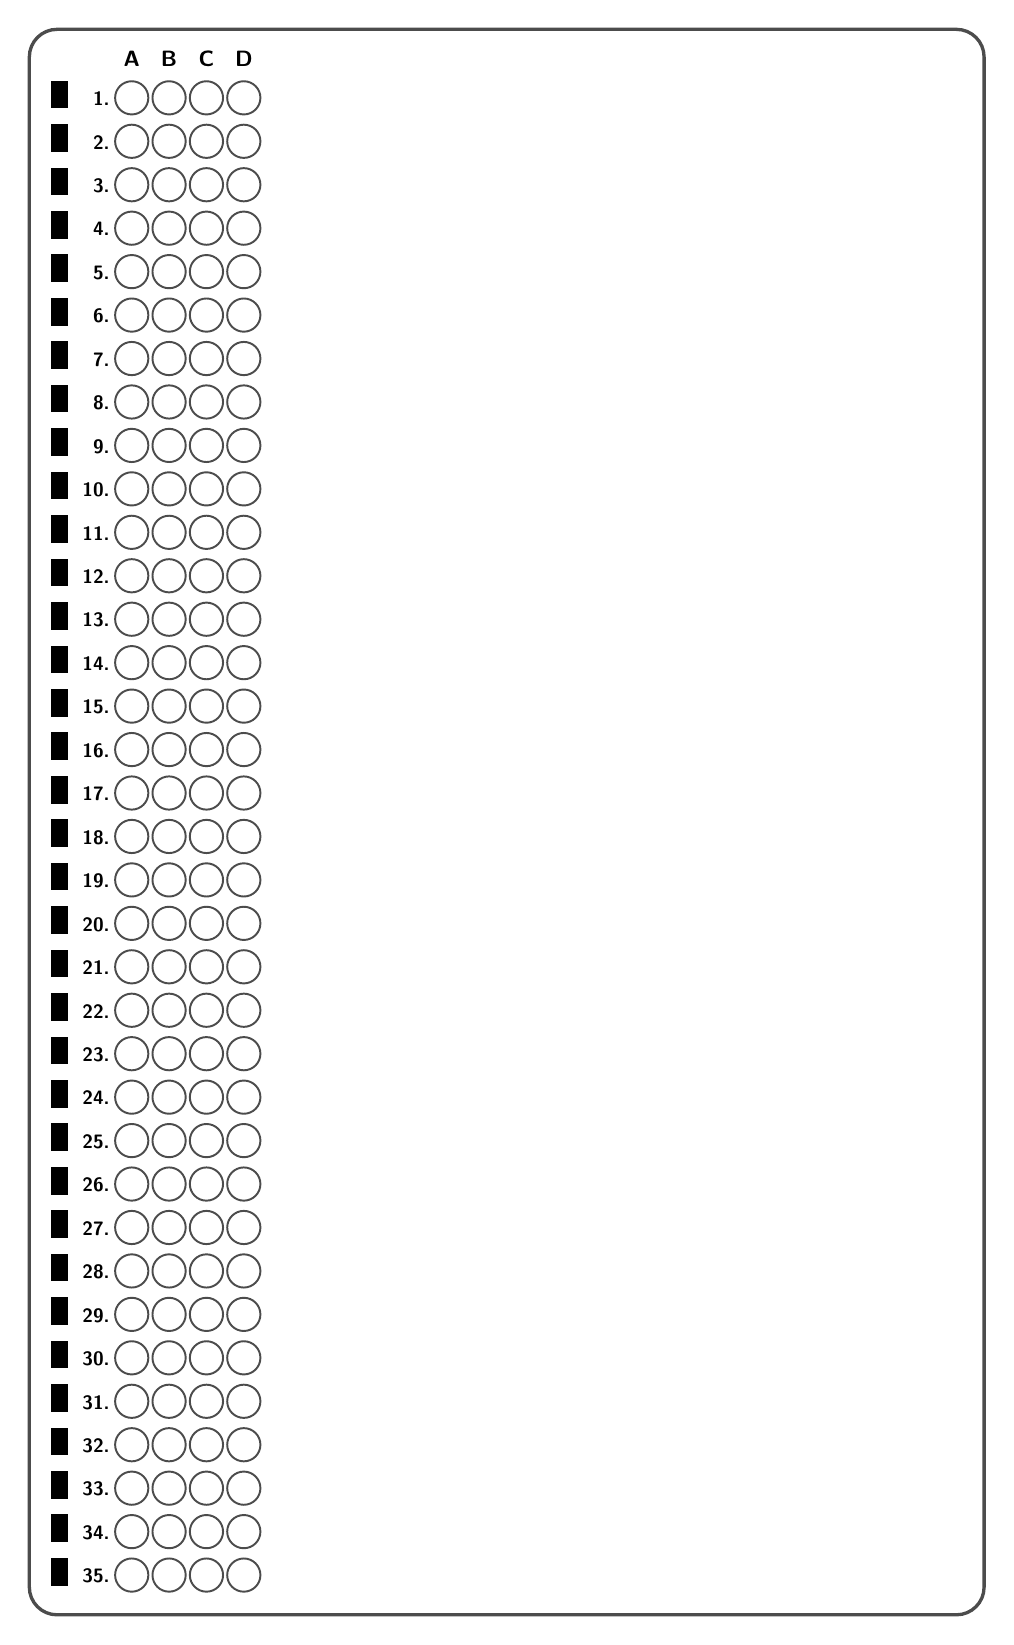
\begin{tikzpicture}
    \node[cuadrocolumna] {
        \HDR
        \foreach \n in {1,...,35}{\Q{\n}}
    };
  \end{tikzpicture}
\end{minipage}%
\hfill
% Columna 2
\begin{minipage}[t]{0.20\textwidth}
  \vspace{0pt}
  \noindent
  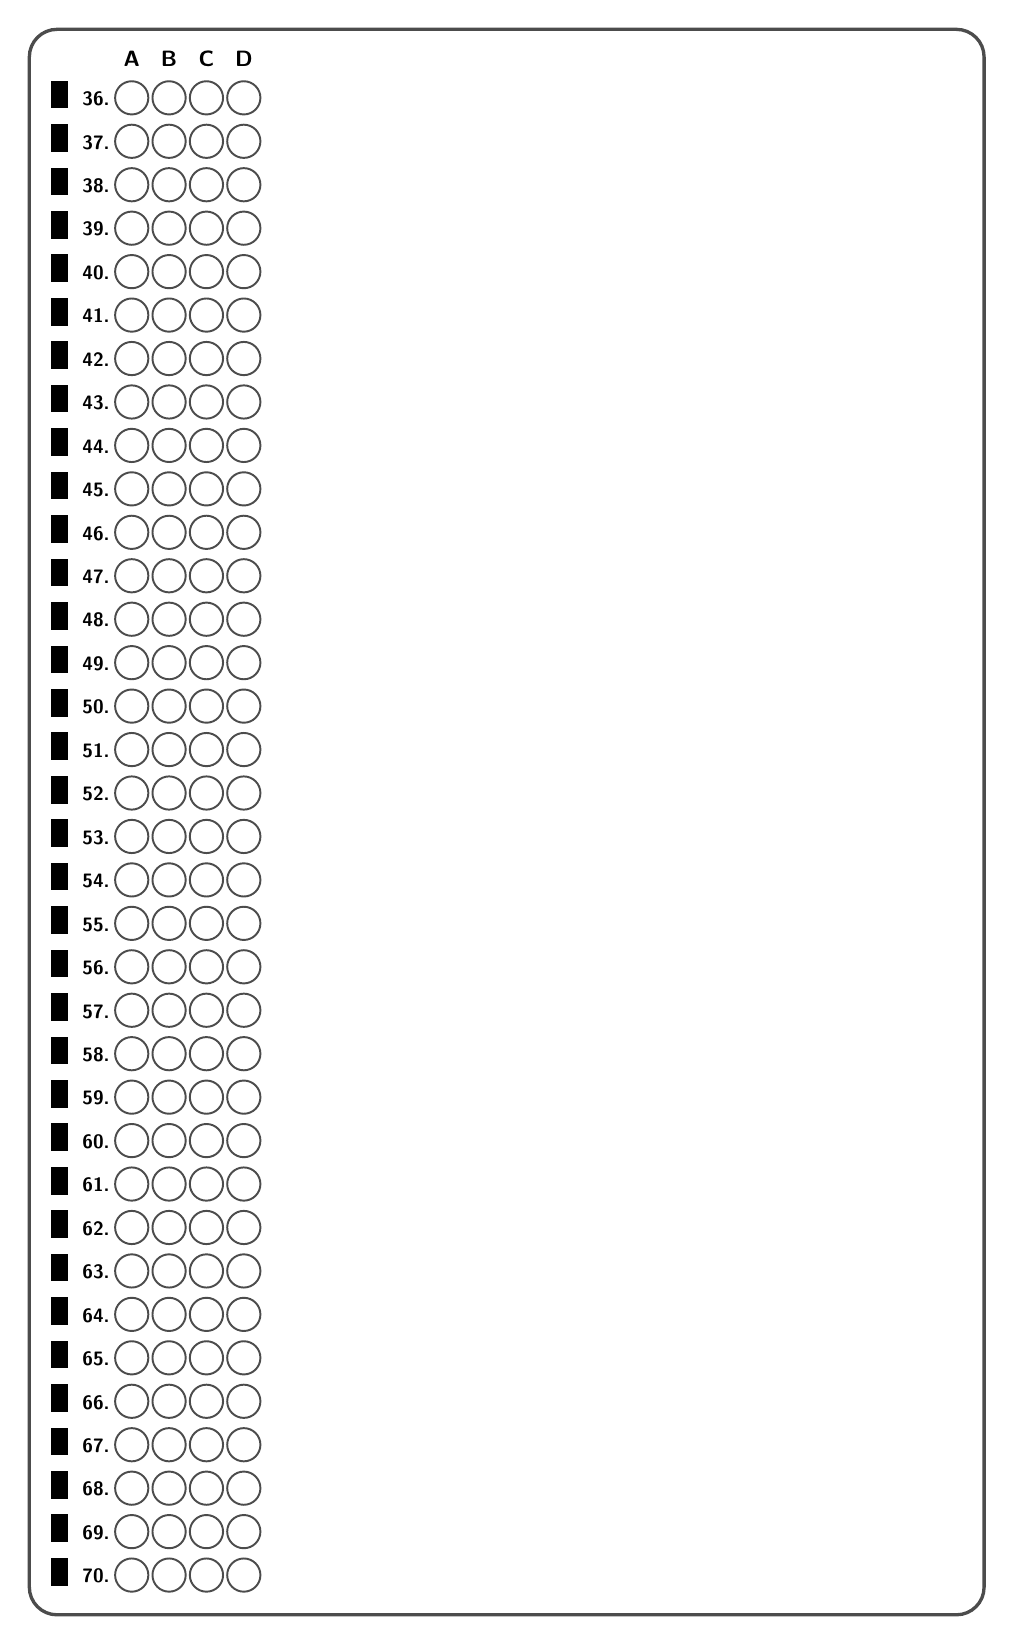
\begin{tikzpicture}
    \node[cuadrocolumna] {
        \HDR
        \foreach \n in {36,...,70}{\Q{\n}}
    };
  \end{tikzpicture}
\end{minipage}%
\hfill
% Columna 3
\begin{minipage}[t]{0.20\textwidth}
  \vspace{0pt}
  \noindent
  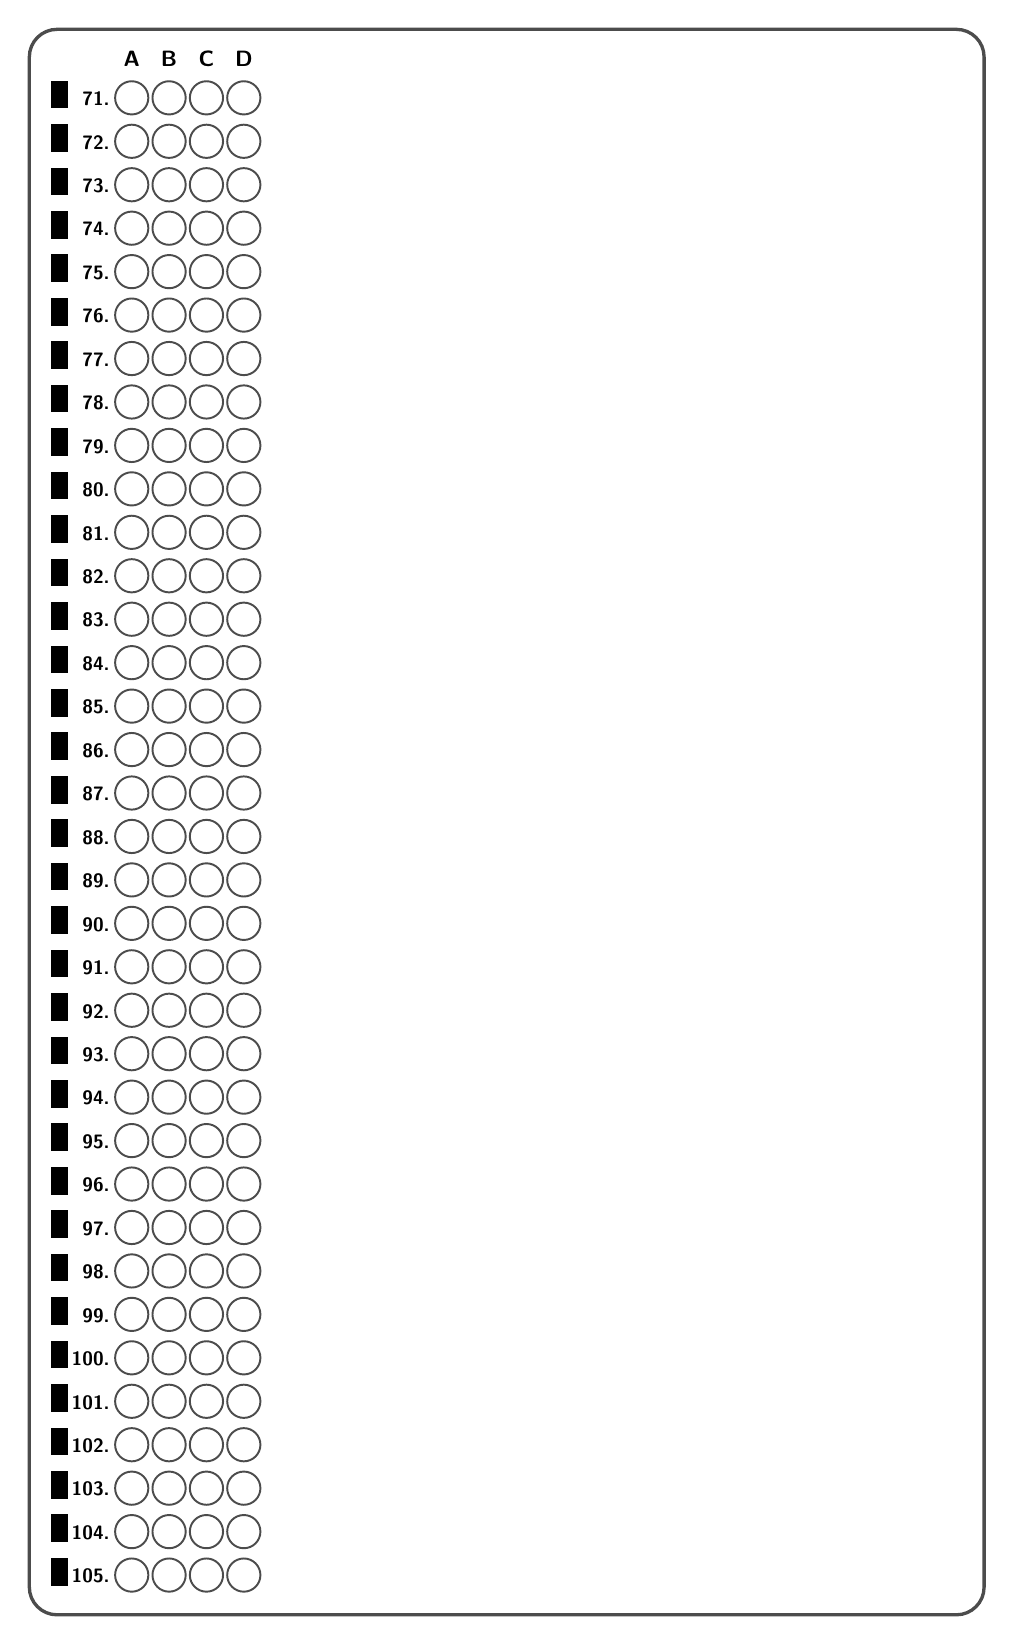
\begin{tikzpicture}
    \node[cuadrocolumna] {
        \HDR
        \foreach \n in {71,...,105}{\Q{\n}}
    };
  \end{tikzpicture}
\end{minipage}%
\hfill
% Columna 4 (MÁS ANCHA para A-H)
\begin{minipage}[t]{0.28\textwidth}
  \vspace{0pt}
  \noindent
  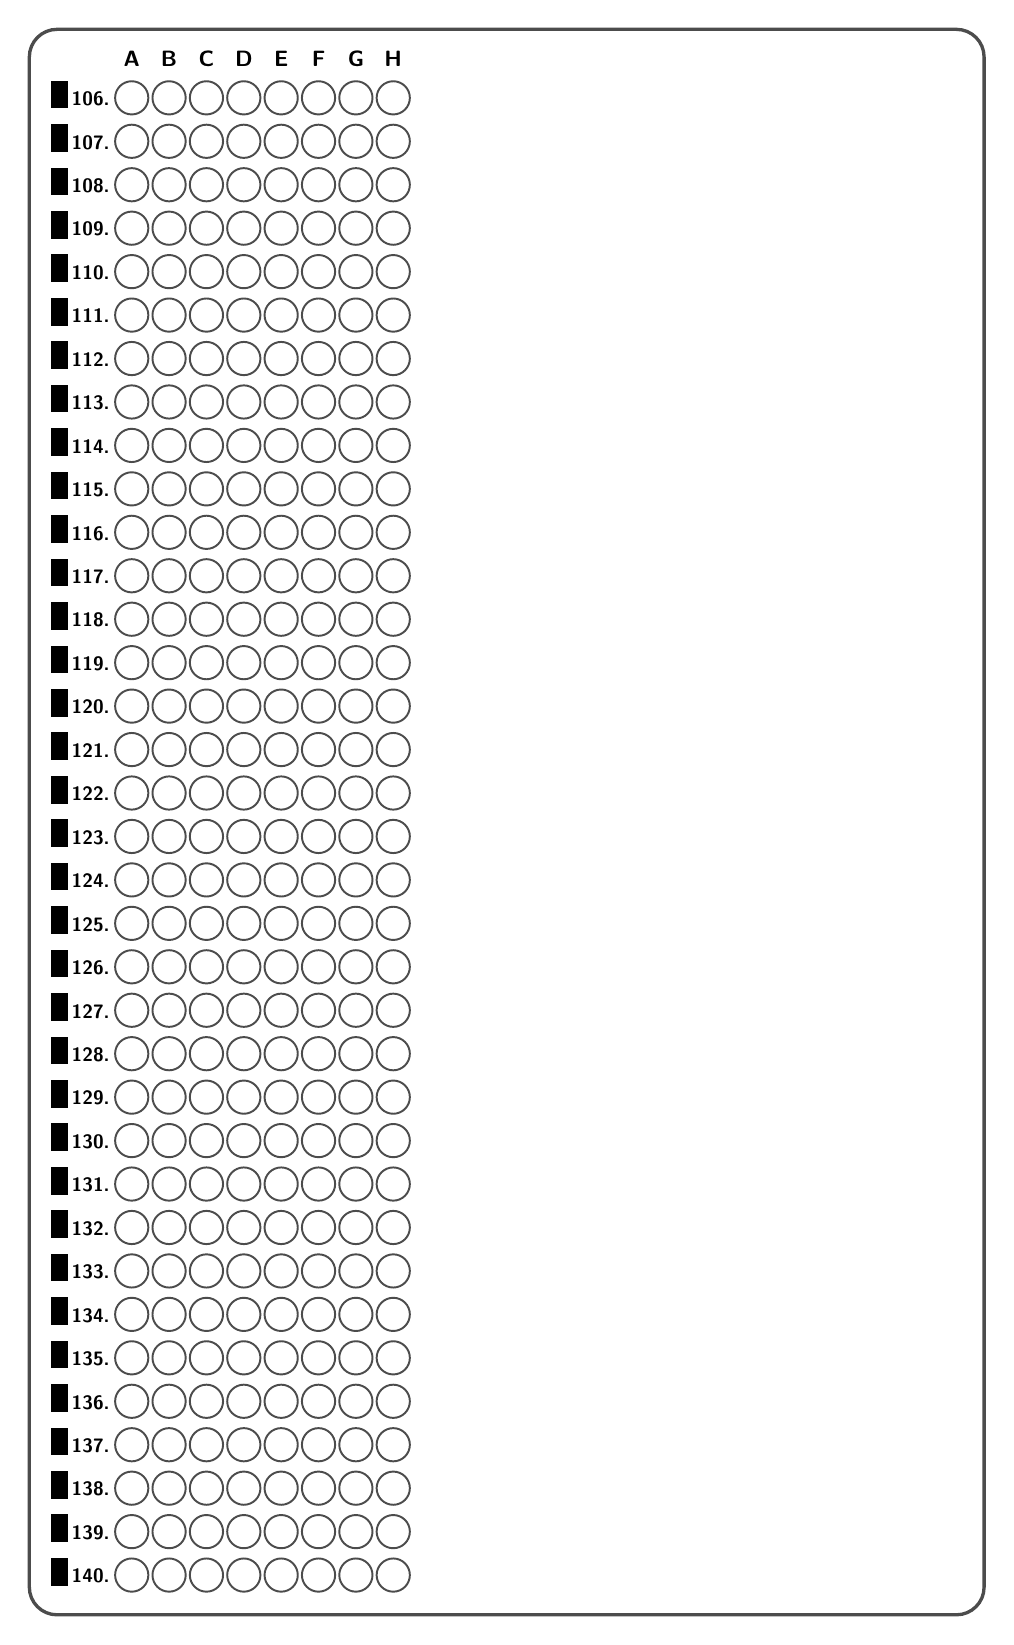
\begin{tikzpicture}
    \node[cuadrocolumna] {
        \HDRH
        \foreach \n in {106,...,140}{\QH{\n}}
    };
  \end{tikzpicture}
\end{minipage}

\end{document}
